\chapter{Team-motivation strategies and personal productivity}
\label{chap:strategies}

In the study, conducted by Dean Spitzer, as many as 50 percent of workers said they only put enough effort into their work to hold onto their jobs. And 84 percent said they could work better —- if they wanted to. \cite{spitzer}

Employee motivation is usually treated as a problem of individual worker. Motivation programs and initiatives try to inspire employees to work harder, but they do nothing about the work conditions that continue to demotivate those same employees.

Thus motivating a team is often more challenging than motivating a single individual. Individuals within teams operate with different goals, values, beliefs, and expectations. Yet the variety of team member personalities can be a positive force if each performer contributes his or her unique capabilities when and where needed \cite{clark-team-motivation} in the correct environment.

\section{Motivation in Daniel Pink's ``Drive"}

Daniel Pink in his book, called ``Drive" shows that much of beliefs about motivation are not true. He also states the problem of a large number of organisations haven't caught up to the new understanding (introduced by Harlow and Deci a few decades ago), and operate from assumptions about human potential and individual performance that are outdated, unexamined, and rooted more in folklore than in science.

\subsubsection{Systems of motivation}

Author suggests to call a system of motivation, that is based on survival needs ``Motivation 1.0". ``Motivation 2.0" was built around external rewards and punishments, so called ``carrots and sticks" method., but it's incompatible with some of the modern thinking, organisations and tasks. The next motivation system is called ``Motivation 3.0."

\begin{wrapfigure}{l}{0.4\textwidth}
    \centering
    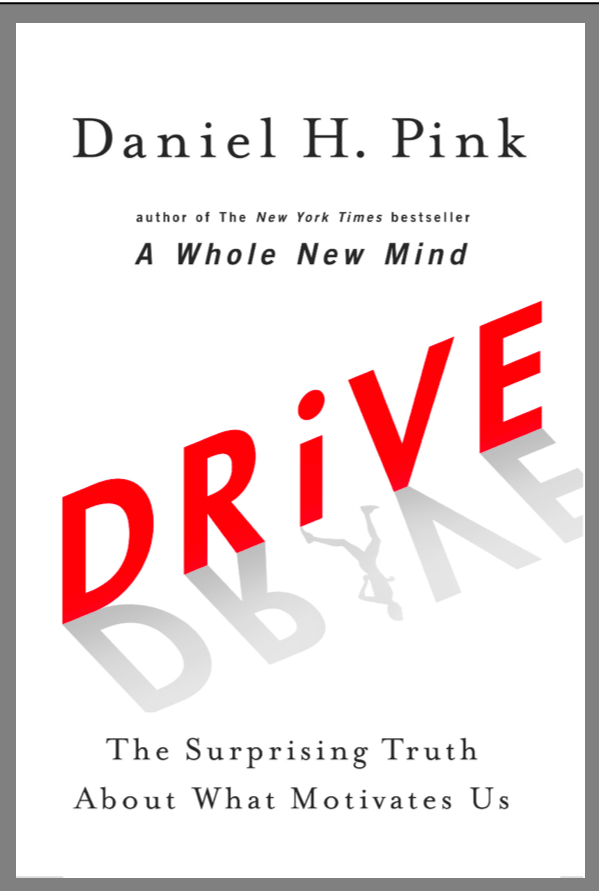
\includegraphics[width=0.4\textwidth]{resources/drive.jpg}
    \caption[Daniel H. Pink, Drive]{Daniel H. Pink, Drive}
\end{wrapfigure}

% EXPERIMENT ON CHILDREN
\textbf{Experiment on inner motivation}

The problem, existing within ``Motivation 2.0" is greatly described by one of Lepper and Greene’s early studies (which they carried out with a third colleague, Robert Nisbett) and has become a classic in the field and among the most cited articles in the motivation literature. The three researchers watched a classroom of preschoolers for several days and identified the children who chose to spend their ``free play" time drawing. Then they fashioned an experiment to test the effect of rewarding an activity these children clearly enjoyed.

The researchers divided the children into three groups. The first was the ``expected- award" group. They showed each of these children a ``Good Player" certificate—adorned with a blue ribbon and featuring the child’s name -- and asked if the child wanted to draw in order to receive the award. The second group was the ``unexpected-award" group. Researchers asked these children simply if they wanted to draw. If they decided to, when the session ended, the researchers handed each child one of the ``Good Player" certificates. The third group was the ``no-award" group. Researchers asked these children if they wanted to draw, but neither promised them a certificate at the beginning nor gave them one at the end.

Two weeks later, back in the classroom, teachers set out paper and markers during the preschool’s free play period while the researchers secretly observed the students. Children previously in the ``unexpected-award" and ``no-award" groups drew just as much, and with the same relish, as they had before the experiment. But children in the first group -- the ones who’d expected and then received an award -- showed much less interest and spent much less time drawing. The Sawyer Effect had taken hold. Even two weeks later, those alluring prizes -- so common in classrooms and cubicles -- had turned play into work.

To be clear, it wasn’t necessarily the rewards themselves that dampened the children’s interest. Remember: When children didn’t expect a reward, receiving one had little impact on their intrinsic motivation. Only contingent rewards -- if you do this, then you’ll get that -- had the negative effect. Why? ``If-then" rewards require people to forfeit some of their autonomy. Like the gentlemen driving carriages for money instead of fun, they’re no longer fully controlling their lives. And that can spring a hole in the bottom of their motivational bucket, draining an activity of its enjoyment.

Lepper and Greene replicated these results in several subsequent experiments with children. As time went on, other researchers found similar results with adults. Over and over again, they discovered that extrinsic rewards—in particular, contingent, expected, ``if-then" rewards—snuffed out the third drive.

These insights proved so controversial -- after all, they called into question a standard practice of most companies and schools -- that in 1999 Deci and two colleagues reanalysed nearly three decades of studies on the subject to confirm the findings. ``Careful consideration of reward effects reported in 128 experiments lead to the conclusion that tangible rewards tend to have a substantially negative effect on intrinsic motivation," they determined. ``When institutions—families, schools, businesses, and athletic teams, for example—focus on the short-term and opt for controlling people’s behaviour," they do considerable long-term damage.

As one leading behavioural science textbook puts it, ``People use rewards expecting to gain the benefit of increasing another person’s motivation and behaviour, but in so doing, they often incur the unintentional and hidden cost of undermining that person’s intrinsic motivation toward the activity."

This is one of the most robust findings in social science -- and also one of the most ignored. Despite the work of a few skilled and passionate popularisers -- in particular, Alfie Kohn, whose prescient 1993 book, Punished by Rewards, lays out a devastating indictment of extrinsic incentives -- we persist in trying to motivate people this way.

% When Carrots and Sticks don't work
\subsubsection{The negative of Motivation 2.0}
When carrots and sticks encounter ones third drive, strange things begin to happen. Traditional ``if-then" rewards can give  less of what a person want: They can extinguish intrinsic motivation, diminish performance, crush creativity, and crowd out good behaviour. They can also give more of what one doesn’t want: They can encourage unethical behaviour, create addictions, and foster short-term thinking (meaning not taking into account long-term outcome).

% When carrots and Sticks work
\subsubsection{The positive of Motivation 2.0}
Carrots and sticks are still can be an effective instrument for rule-based routine tasks -- because there’s little intrinsic motivation and not much creativity involved. And they can be more effective still if those giving such rewards offer a rationale for why the task is necessary, acknowledge that it’s boring, and allow people autonomy over how they complete it.
% засунуть сюда схему
For non-routine conceptual tasks, rewards are more perilous -- particularly those of the ``if-then" variety. But ``now that" rewards -- noncontingent rewards given after a task is complete -- can sometimes be okay for more creative, right-brain work, especially if they provide useful information about performance.

% Personality type
\subsubsection{Personality types and motivation}
Daniel Pink also states, that Motivation 2.0 depended on and fostered Type X behaviour -- behaviour fueled more by extrinsic desires than intrinsic ones and concerned less with the inherent satisfaction of an activity and more with the external rewards to which an activity leads. Motivation 3.0, the upgrade that’s necessary for the smooth functioning of twenty-first-century business, depends on and fosters Type I behaviour. Type I behaviour concerns itself less with the external rewards an activity brings and more with the inherent satisfaction of the activity itself. For professional success and personal fulfilment, one need to move himself from Type X to Type I. Positevly, Type I people are made, not born -- and Type I behaviour leads to stronger performance, greater health, and higher overall well-being.

% Autonomy
\subsubsection{Motivation}
A person naturally seeks to be autonomous and self-directed. Unfortunately, circumstances -- including outdated notions of ``management" -- often conspire to change that default setting and turn a person from Type I to Type X. To encourage Type I behaviour, and the high performance it enables, the first requirement is autonomy. People need autonomy over task (what they do), time (when they do it), team (who they do it with), and technique (how they do it). Companies that offer autonomy, sometimes in radical doses, are outperforming their competitors.

% Mastery
\subsubsection{Mastery}
While Motivation 2.0 required compliance, Motivation 3.0 demands engagement. Only engagement can produce mastery --becoming better at something that matters. And the pursuit of mastery, an important but often dormant part of the third drive, has become essential to making one’s way in the economy. Mastery begins with ``flow"-optimal experiences (to be considered in detail in section \ref{sec:flow}) when the challenges faced are exquisitely matched to abilities. Smart workplaces therefore supplement day-to-day activities with ``Goldilocks tasks" -- not too hard and not too easy. But mastery also abides by three peculiar rules. Mastery is a mindset: It requires the capacity to see abilities not as finite, but as infinitely improvable. Mastery is a pain: It demands effort, grit, and deliberate practice. And mastery is an asymptote: It’s impossible to fully realise, which makes it simultaneously frustrating and alluring.

% Purpose
\subsubsection{Purpose}
Humans, by their nature, seek purpose -- a cause greater and more enduring than themselves. But traditional businesses have long considered purpose ornamental -- a perfectly nice accessory, so long as it didn’t get in the way of the important things. But that’s changing -- thanks in part to the rising tide of aging baby boomers reckoning with their own mortality. In Motivation 3.0, purpose maximisation is taking its place alongside profit maximisation as an aspiration and a guiding principle. Within organisations, this new ``purpose motive" is expressing itself in three ways: in goals that use profit to reach purpose; in words that emphasize more than self-interest; and in policies that allow people to pursue purpose on their own terms. This move to accompany profit maximisation with purpose maximisation has the potential to rejuvenate our businesses and remake our world.


% GOALS (LOOK DEEPER)
\subsubsection{Goals}
So how to deal with steps (goals) definition. Of course, all goals are not created equal. Goals and extrinsic rewards aren’t inherently corrupting. But goals are more toxic than Motivation 2.0 recognises. In fact, the business school professors suggest they should come with their own warning label: Goals may cause systematic problems for organisations due to narrowed focus, unethical behaviour, increased risk taking, decreased cooperation, and decreased intrinsic motivation. One should use care when applying goals in organisation.

\begin{compactitem}
\item Offering a rationale for why the task is necessary. A job that’s not inherently interesting can become more meaningful, and therefore more engaging, if it’s part of a larger purpose. For example: ``Explain why this poster is so important and why sending it out now is critical to your organisation’s mission."
\item Acknowledge that the task is boring. This is an act of empathy, of course. And the acknowledgment will help people understand why this is the rare instance when ``if-then" rewards are part of how organisation operates.
\item Allow people to complete the task their own way. Think autonomy, not control. State the outcome you need. But instead of specifying precisely the way to reach it—how each poster must be rolled and how each mailing label must be affixed—give them freedom over how they do the job.
\end{compactitem}

% DO's and DONT'S
\textbf{Do's and dont's}
\begin{compactitem}
\item  Offering an ``if-then" reward to the design staff. A one shouldn't stride into the office and announce: ``If you come up with a poster that rocks my world or that boosts attendance over last year, then you’ll get a ten-percent bonus." Although that motivational approach is common in organisations all over the world, it’s a recipe for reduced performance. Creating a poster isn’t routine. It requires conceptual, breakthrough, artistic thinking. The best approach is to have already established the conditions of a genuinely motivating environment. The baseline rewards must be sufficient. That is, the team’s basic compensation must be adequate and fair --particularly compared with people doing
\item Similar work for similar organisations. A nonprofit must be a congenial place to work. And the people on team must have autonomy, they must have ample opportunity to pursue mastery, and their daily duties must relate to a larger purpose. If these elements are in place, the best strategy is to provide a sense of urgency and significance—and then get out of the talent’s way. But one may still be able to boost performance a bit -- more for future tasks than for this one -- through the delicate use of rewards. Efforts will backfire unless the rewards offered meet one essential requirement. 
\item The essential requirement: Any extrinsic reward should be unexpected and offered only after the task is complete.
Holding out a prize at the beginning of a project -- and offering it as a contingency -- will inevitably focus people’s attention on obtaining the reward rather than on attacking the problem. But introducing the subject of rewards after the job is done is less risky.
In other words, where ``if-then" rewards are a mistake, shift to ``now that" rewards -- as in ``Now that you’ve finished the poster and it turned out so well, I’d like to celebrate by taking you out to lunch." 
As Deci and his colleagues explain, ``If tangible rewards are given unexpectedly to people after they have finished a task, the rewards are less likely to be experienced as the reason for doing the task and are thus less likely to be detrimental to intrinsic motivation." So when the poster turns out great, one could buy the design team a case of beer or even hand them a cash bonus without snuffing their creativity. The team didn’t expect any extras and getting them didn’t hinge on a particular outcome. A person simply offers his appreciation for their stellar work. But repeated ``now that" bonuses can quickly become expected ``if-then" entitlements—which can ultimately crater effective performance.
A firmer motivational footing is created if follow two additional principles.
\subitem Consider nontangible rewards. Praise and positive feedback are much less corrosive than cash and trophies. In fact, in Deci’s original experiments, and in his subsequent analysis of other studies, he found that ``positive feedback can have an enhancing effect on intrinsic motivation."
\subitem Provide useful information. Amabile has found that while controlling extrinsic motivators can clobber creativity, ``informational or enabling motivators can be conducive" to it. In the workplace, people are thirsting to learn about how they’re doing, but only if the information isn’t a tacit effort to manipulate their behaviour. The following shouldn't be permitted: ``That poster was perfect. You did it exactly the way I asked." Instead, people should be given a meaningful information about their work. The more feedback focuses on specifics (``great use of colour") -- and the more the praise is about effort and strategy rather than about achieving a particular outcome -- the more effective it can be.
\end{compactitem}

\section{Goal commitment formula by Richard Clark}

While Daniel Pink provides a distinction between different types of tasks and motivation behind them, Richard Clark did a great study on the components of goal commitment. 

Cark's paper quotes Hogan Curphy and Hogan review of leadership studies: found that only about 30 percent of line managers are able to adequately motivate the people who report to them. They imply that in most circumstances, motivation accounts for about half of all performance results.

The late Tom Gilbert, one of the clearest thinkers in performance improvement, was fond of saying that when two people had equal abilities, the enthusiastic member of the pair would achieve about 70 percent more than the unenthusiastic person. Even more troubling is that evidence that a majority of the published studies of organisational development strategies that report measured increases in motivation are fatally flawed. Strategies that may not work as powerfully or as consistently as claimed include popular employee empowerment strategies, contests, job redesign, leaderless teams and various performance recognition techniques.

In the CANE model, motivation is defined as two interlinked processes. The first process leads us to make a commitment to a performance goal and persist the face of distractions from appealing but less important alternative goals. The second motivation process is concerned with the amount and quality of the “mental effort” people invest in achieving the knowledge component of performance goals. These two motivation processes, committed, active and sustained goal pursuit on the one hand, and necessary mental effort to tackle goal-related problems, on the other hand, are the primary motivation goals in the CANE model.

% include a scheme

\begin{figure}[ht]

    \begin{minipage}[t]{0.5\linewidth}
    {\bf KNOWLEDGE}\\
    Makes it possible to:\\
    
    {\small
    Understand goals\\
    Develop/implement plans to reach goals\\
    Monitor progress towards goals\\
    Revise and improve plans
    }
    \end{minipage}
    \begin{minipage}[t]{0.5\linewidth}
    {\bf MOTIVATION}\\
    Makes it possible to:\\
    
    {\small
    Make a strong commitment to goals\\
    Persist with plans and goals when distracted\\
    Monitor goal value and personal confidence\\
    Invest necessary mental effort in plans
    }
    \end{minipage}
    
    \caption{Knowledge and motivation systems}

\end{figure}

In today’s complex work environments the variety of job tasks that confront all of us change constantly over time. We cannot commit ourselves equally to all tasks. We must prioritise and focus on important tasks in order to be successful. Commitment problems happen when people resist assigning adequate priority to important job tasks. Research on motivation suggests that people with commitment problems may avoid a task altogether and/or argue that the task is less important than some other set of tasks.

\begin{figure}[b]
	\centering
	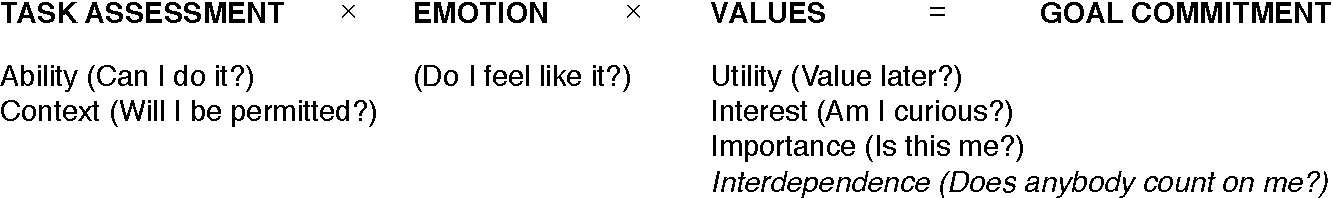
\includegraphics[width=0.8\textwidth]{resources/goal-commitment.pdf}
	\caption[CANE Model of Factors Influencing Goal Commitment]{CANE Model of Factors Influencing Goal Commitment}
\end{figure}

Three factors have been found to increase (or decrease) work goal commitment. The first factor is {\bf ``task assessment".} All of us will analyse any task we are assigned to determine whether we can successfully complete the task. We all tend to ask ourselves two questions about new tasks - ``Can I do it?" and “Will I be permitted to do it?”. If we think that we have the ability to accomplish the goal and that we will be permitted to accomplish it, our commitment will increase. If we doubt our ability or the organisation’s willingness to let us use our skills, commitment will decrease.

{\bf Emotion and commitment.} The second factor influencing commitment is our mood or emotions. All positive emotions facilitate commitment and all powerful, negative emotions discourage goal commitment. This may seem like a minor issue but for temperamental people or in organisations where pressure is high and/or change is constant, negative emotional undercurrents can be strong. Angry or depressed people find it nearly impossible to make a commitment to work goals.

{\bf Values and commitment.} The final factor that influences the strength of goal commitment is our personal value in the goal. It is my experience that values are the most important element in increasing or decreasing the strength of our commitments. Psychologists now have good evidence that the most important value at work is our belief about whether the achievement of a work goal will increase our personal control or effectiveness (Shapiro et al, 1996; Locke and Latham, 1990). The more we believe that achievement of a work goal will make us more successful, the higher our level of commitment to the goal. The reverse is also true. Few of us will give a high priority to tasks that we sincerely believe will lead us to fail or be perceived as incompetent Utility, Interest and Importance Values.

%CANE Model of Factors Influencing Goal Commitment

\subsubsection{Task Assessment Solutions}

Solving task assessment problems require that we convince people that they can do a job and that existing barriers to their performance will be removed. Pointing out familiar, past examples of job performance that are similar to the new task helps increase confidence. In addition, job aids can bolster confidence. Involving staff in the elimination of any procedural or policy barriers to performance reduces resistance based on task assessment. The service technicians had excellent job aids which increased their confidence about the form task. The key element here is to persuade or empower people to believe that they can succeed at the task they are avoiding. Bandura provides extensive examples of solutions in this area.

\subsubsection{Mood solutions.}

Mood problems often take more time to develop than task assessment or value problems. I find mood problems to be key elements in organisations where a major culture or job change is occurring. This is particularly true in organisations that are changing from a “civil service” to a business culture.

Solutions that have been found to change mood states have included listening to positive mood music; writing or telling about a positive mood-related experience; watching a movie or listening to stories that emphasize positive mood states; and emotion control training through ``environmental control strategies" including the choice of how we complete work tasks, adjusting work space and ``positive self talk".

\subsubsection{Value solutions}

The solution to most commitment problems and opportunities is to convince people that completing the task they are resisting will make them more effective and/or perceived as more effective. People simply will not do what they believe will make them less effective or less successful. Many people are suspicious of change simply because they feel that they will be perceived as less effective under novel, negative or uncertain conditions. They must be convinced that if they commit themselves to the avoided task(s) they will become significantly more effective or successful. The specific solution that accomplishes this goal may be quite different for different individuals and work cultures. Some organisations have adopted various ``employee empowerment" solutions to value problems. In many empowerment settings staff are asked to choose their own work goals in order to get them to value their work. There is good research evidence that this is not necessary.

In cases where participatory goal setting is not possible, they find that value for the goal is enhanced if people perceive the goal to be: 1) assigned by a legitimate, trusted authority with an ``inspiring vision" that reflects a ``convincing rationale" for the goal (importance value), and who; 2) provides expectation of outstanding performance (importance value) and gives: 3) ``ownership" to individuals and teams for specific tasks (interest value); 4) expresses confidence in individual and team capabilities (interest value) while; 5) providing feedback on progress that includes recognition for success and supportive but corrective suggestions for mistakes (utility value).

\subsubsection{Motivation Solutions}

Value problems are often multi-level issues in an organisation. In this organisation, there were a number of beliefs and patterns that had to be considered. The mangers of the technicians had their own motivational issues to handle. For example, the senior manager acting as sponsor for the motivation project placed a number of constraints on a value solution for the technicians.

Two types of motivation are important at work, persistence and mental effort. Commitment (persistence at a task) is increased by convincing people that: a) the organisation will remove unnecessary barriers; b) that achievement of the work goal will make the person more personally effective; and c) that the manager requesting the goal is credible, trustworthy, optimistic (about the person or team’s ability to achieve the goal), able to clearly communicate the vision connected to the goal and willing to give ownership for the accomplishment. Mental effort is enhanced by insuring that the goal assigned is very challenging. Managers must work with people to adjust their confidence level whenever they become over confident (and thus refuse to take responsibility for errors or poor performance) or under confident (and thus find an excuse to procrastinate or avoid the goal altogether).

\section{Gamification}

Following the success of the location-based service Foursquare, the idea of using game design elements in non-game contexts to motivate and increase user activity and retention has rapidly gained traction in interaction design and digital marketing. Under the moniker ``gamification", this idea is spawning an intense public debate as well as numerous applications – ranging across productivity, finance, health, education, sustainability, as well as news and entertainment media. Several vendors now offer ``gamification" as a software service layer of reward and reputation systems with points, badges, levels and leader boards.

This commercial deployment of `gamified' applications to large audiences potentially promises new, interesting lines of inquiry and data sources for human-computer interaction (HCI) and game studies – and indeed, ``gamification" is increasingly catching the attention of researchers.

Whereas ``serious game" describes the design of full-fledged games for non-entertainment purposes, ``gamified" applications merely incorporate elements of games (or game ``atoms" [10]). Of course, the boundary between ``game" and ``artifact with game elements" can often be blurry – is Foursquare a game or a ``gamified" application? To complicate matters, this boundary is empirical, subjective and social: Whether you and your friends `play' or `use' Foursquare depends on your (negotiated) focus, perceptions and enactments. The addition of one informal rule or shared goal by a group of users may turn a `merely' `gamified' application into a `full' game. Within game studies, there is an increasing acknowledgement that any definition of `games' has to go beyond properties of the game artifact to include these situated, socially constructed meanings. For the present purpose, this means that (a) artifactual as well as social elements of games need to be considered, and (b) artifactual elements should be conceived more in terms of affording gameful interpretations and enactments, rather than being gameful. Indeed, the characteristic of `gamified' applications might be that compared to games, they afford a more fragile, unstable `flicker' of experiences and enactments between playful, gameful, and other, more instrumental-functionalist modes.

% table goes here

As can be seen, this ‘level model’ distinguishes interface design patterns from game design patterns or game mechanics. Although they relate to the shared concept of pattern languages, unlike interface design patterns, neither game mechanics nor game design patterns refer to (prototypical) implemented solutions; both can be implemented with many different interface elements. Therefore, they are more abstract and thus treated as distinct.

So to restate, whereas serious games fulfill all necessary and sufficient conditions for being a game, “gamified” applications merely use several design elements from games. Seen from the perspective of the designer, what distinguishes “gamification” from ‘regular’ entertainment games and serious games is that they are built with the intention of a system that includes elements from games, not a full ‘game proper’. From the user perspective, such systems entailing design elements from games can then be enacted and experienced as ‘games proper’, gameful, playful, or otherwise – this instability or openness is what sets them apart from ‘games proper’ for users.

Similar to serious games, ``gamification" uses elements of games for purposes other than their normal expected use as part of an entertainment game. Now `normal use' is a socially, historically and culturally contingent category. However, it is reasonable to assume that entertainment currently constitutes the prevalent expected use of games. Likewise, joy of use, engagement, or more generally speaking, improvement of the user experience represent the currently predominant use cases of ``gamification".

To summarize: ``Gamification" refers to
\begin{compactitem}
\item the use (rather than the extension) of
\item design (rather than game-based technology or other game-
related practices)
\item elements (rather than full-fledged games)
\item characteristic for games (rather than play or playfulness)
\item in non-game contexts (regardless of specific usage intentions, contexts, or media of implementation).
\end{compactitem}


This definition contrasts ``gamification" against other related concepts via the two dimensions of playing / gaming and parts / whole. Both games and serious games can be differentiated from ``gamification" through the parts/whole dimension. Playful design and toys can be differentiated through the playing/gaming dimension.


\subsection{Appropriate game mechanics for the basic project management}

The following list of requirements for successful productivity application was conducted (the full list of game mechanics can be found in appendix \ref{chap:gamemech}):

\begin{compactitem}
\item ``Achievement" game mechanics supports desire to perform tasks
\item ``Pride" game mechanics supports retention of joy from executed tasks
\item ``Avoidance" game mechanics helps a person return to application
\item ``Cascading Information Theory" allows to introduce difficult concepts of GTD (Getting Things Done) and increase a person’s activity in the application
\item ``Communal Discovery" is used in collaborative tasks / task delegation
\item ``Progression Dynamic" helps visualize improvement and progress to a goal.
\end{compactitem}

\section{Mihaly Csikszentmihalyi's concept of ``Flow"}
\label{sec:flow}

The author has been studying for over 20 years the states of optimal experience -- those times when people report feelings of concentration and deep enjoyment. These investigations have revealed that what makes experience genuinely satisfying is a state of consciousness called flow--a state of concentration so focused that it amounts to absolute absorption in an activity. 

Everyone experiences flow from time to time and will recognise its characteristics: people typically feel strong, alert, in effortless control, unselfconscious, and at the peak of their abilities. Both a sense of time and emotional problems seem to disappear, and there is an exhilarating feeling of transcendence. Flow: The Psychology of Optimal Experience describes how this pleasurable state can be controlled, and not just left to chance, by setting ourselves challenges -- tasks that are neither too difficult nor too simple for our abilities. With such goals, we learn to order the information that enters consciousness and thereby improve the quality of our lives.

\begin{figure}[t]
	\centering
	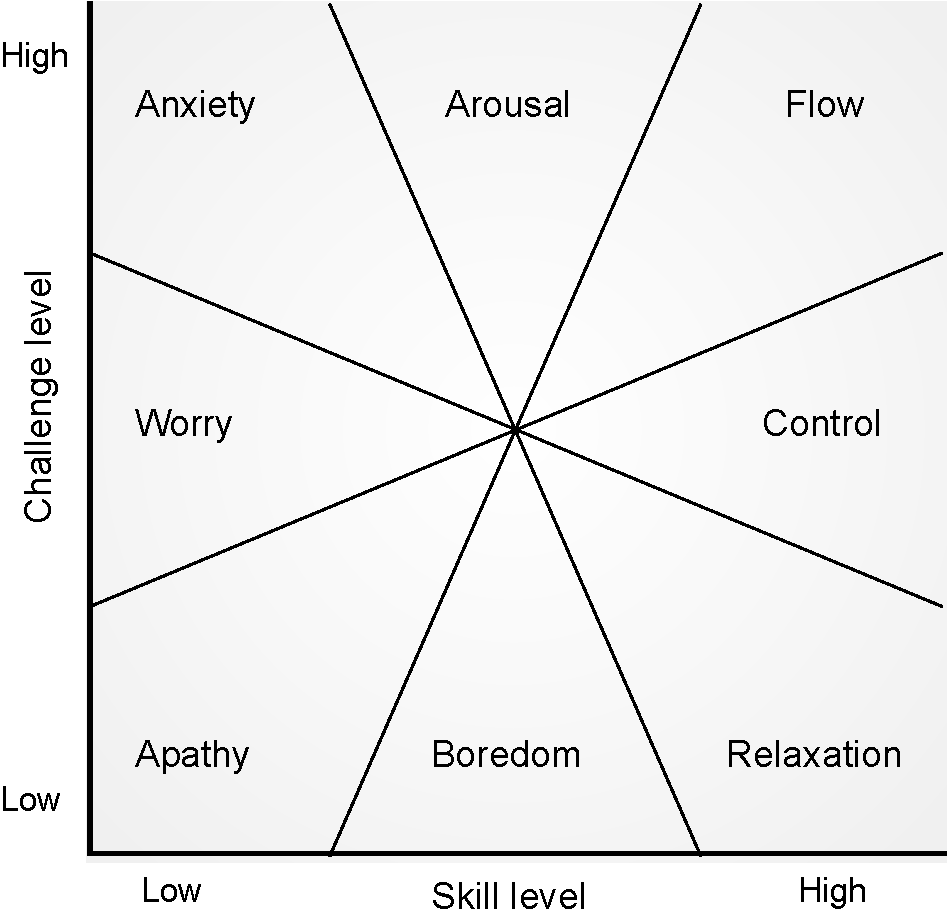
\includegraphics[width=0.7\textwidth]{resources/flow.pdf}
	\caption[Challenge to Skill Relation]{Challenge to Skill Relation}
\end{figure}

The studies have suggested that the phenomenology of enjoyment has eight major components. When people reflect on how it feels when their experience is most positive, they mention at least one, and often all, of the following:
\begin{compactitem}
\item We confront tasks we have a chance of completing;
\item We must be able to concentrate on what we are doing; 
\item The task has clear goals;
\item The task provides immediate feedback;
\item One acts with deep, but effortless involvement, that removes from awareness the worries and frustrations
of everyday life;
\item One exercises a sense of control over their actions;
\item Concern for the self disappears, yet, paradoxically
the sense of self emerges stronger after the flow experience is over; and
\item The sense of duration of time is altered.
The combination of all these elements causes a sense of deep enjoyment that is so rewarding people feel that expending a great deal of energy is worthwhile simply to be able to feel it.
\end{compactitem}

\textbf{A Challenging Activity that Requires Skills}

Optimal experiences are reported to occur within sequences of activities that are goal-directed and bounded by rules--activities that require the investment of psychic energy (attention) and that could not be done without skills. Please note that activities do not need to be physical and skills also need not be physical skills. For instance, the most frequently mentioned enjoyable activity the world over was reading, followed closely by being with other people. For those who do not have the right skills, an activity is not challenging; it is simply meaningless. Challenges of competition were found to be stimulating and enjoyable. But when beating the opponent takes precedence in the mind over performing as well as possible, enjoyment tends to disappear. Competition is enjoyable only when it is a means to perfect one's skills; when it becomes an end in itself, it ceases to be fun.

% Include graphic of the flow

\textbf{The Merging of Action and Awareness}

One of the most universal and distinctive features of optimal experience is the people become so involved in what they are doing that the activity becomes spontaneous, almost automatic; they stop being aware of themselves as separate from the actions they are performing. It often requires strenous physical exertion, or highly disciplined mental activity to enter a continuous flow.

\textbf{Clear Goals and Feedback}

Unless a person learns to set goals and to recognize and gauge feedback in their activities, she will not enjoy them. For activities that are creative or open-ended in nature, a person must develop a strong sense of what she intends to do or negotiate goals and rules during the activity. These goals and rules provide benchmarks for feedback. The kind of feedback we work toward is in, and of itself, often unimportant. What makes feedback valuable is the symbolic message it contains: that I have succeeded in my goal.

\textbf{Concentration on the Task at Hand}

One of the most frequently mentioned dimensions of the flow experience is that, while it lasts, one is able to forget all the unpleasant aspects of life. The task requires such concentration that only a very select range of information can be allowed into awareness.

\textbf{The Paradox of Control}

The flow experience is typically described as involving a sense of control--or more precisely, as lacking the sense of worry about losing control that is typical in many situations of normal life. What people enjoy is not the sense of being in control, but the sense of exercising control in difficult situations. However, when a person becomes dependent on the ability to control an enjoyable activity then he loses the ultimate control: the freedom to determine the content of consciousness. While experiences are capable of improving the quality of existence by creating order in the mind, they can also become addictive, at which point the self becomes captive of a certain kind of order, and is then unwilling to cope with the ambiguities of life.

\textbf{The Loss of Self-Consciousness}

When in a flow experience, what slips below the threshold of awareness is the concept of self, the information we use to represent to ourselves who we are. And being able to forget temporarily who we are seems to be very enjoyable. When not preoccupied with our selves, we actually have a chance to expand the concept of who we are. Loss of self-consciousness can lead to self-transcendence, to a feeling that the boundaries of our being have been pushed forward.

\textbf{The Transformation of Time}

One of the most common descriptions of optimal experience is that time no longer seems to pass the way it ordinarily does. Generally, after the experience we do not know where the time went; however, during the actual experience, time seems to stand still.

The key element of an optimal experience is that it is an end in itself. It is an autotelic experience. The term ``autotelic" derives from two Greek words, ``auto" meaning self, and ``telos" meaning goal. It refers to a self-contained activity, one that is done not with the expectation of some future benefit, but simply because the doing itself is the reward. Teaching children in order to turn them into good citizens is not autotelic, whereas teaching them because one enjoys interacting with children is. Most enjoyable activities are not natural; they demand an effort that initially one is reluctant to make. But once the interaction starts to provide feedback to the person's skills, it usually begins to be intrinsically rewarding.

Flow in the family context has five characteristics:
\begin{compactitem}
\item \textbf{Clarity:} children know what parents expect from them; 
\item \textbf{Centering:} children know that their parents are interested in what they are doing in the present;
\item \textbf{Choice:} children feel that they have a variety of possibilities from which to choose;
\item \textbf{Commitment:} trust that allows the child to feel comfortable enough to set aside the shield of defenses and become unself-consciously involved; and
\item \textbf{Challenge:} providing increasingly complex opportunities for action.
\end{compactitem}

\section{General guidelines}

These guidelines were combined with advices from ``Winning without losing" by Martin Bjergegaard, Jordan Milne.

Personal guidelines:

\begin{compactenum}

\item A list of things, that take your time, but don't contribute neither to effectiveness nor to happiness is effective
\item It is OK to force yourself to do things that engage
\item A person should value and appreciate things you did today
\item Often visit the open air
\item Know your plan B (maybe secondary tasks for today)
\item Split the day between different spheres of life, 8-8-8
\item Happiness is to stay active and not to be tired in taking new tasks, which help you develop and learn
\item Don't create a long business-plans
\item See the big picture
\item Don't micromanage, let others do their work
\item Don't try to get everything done, just the important
\item Lucid respites are important
\item A list for today (fixed length)
\item Lean
\item Not a schedule, but inspirationz
\item It is better to solve bad tasks at first

\end{compactenum}

% Scheme of the effectiveness
